\documentclass[8pt,letter]{extarticle}     % Necessary to make small margin an small text paper.
\usepackage[utf8]{inputenc}	                % UTF-8 characters.
\usepackage[landscape, margin=1cm, bmargin=0.5cm, includefoot, footskip=0.5cm]{geometry}            % Necessary for landscape paper.
\usepackage[textsize=tiny]{todonotes}       % Necessary for small margins.
\usepackage{enumitem}                       % Necessary for personalized lists.
\usepackage{mdframed}                       % Necessary for dark gray boxes.
\usepackage{mathtools}                      % More compact math.
\usepackage{amsthm}                         % Necessary for theorem boxes.
\usepackage{amssymb}						% Necessary for mathbb symbols.
\usepackage{multicol,multirow}              % Necessary for multi column format.
\usepackage{subfiles}						% Necessary for multiple subfiles
\usepackage{tabularx}						% Necessary for full-column tables 
\usepackage{bm}								% Necessary for bold math with \pbm{...}
\usepackage{xcolor}							% Necessary for custom colors. 
\usepackage{graphicx}
\usepackage{accents}						% Necessary for doublehat
\usepackage{pgfplots}
\usepackage{fancyhdr}						% Necessary for header/footer settings

% Header / Footer settings
\pagestyle{fancy}
\renewcommand{\headrulewidth}{0pt}
\rhead{} 
\lhead{} 
\chead{} 
\cfoot{AP Calculus BC $\cdot$ Cheat Sheet}
\lfoot{}
\rfoot{Page \thepage}


% For Figures
\usetikzlibrary{decorations.markings}
\pgfplotsset{compat=1.11}



%---------------------------------------------------%
% Environments
%---------------------------------------------------%

% For Claims 
\mdtheorem [%
		backgroundcolor	= black!10,%
		topline			= false,%
		bottomline	= false,%
		leftline		= false,%
		rightline		= false%
		]{boxclaim}{Claim}[section]
		%comment [section] for global numbering


% For Definitions
\newmdtheoremenv [%
		backgroundcolor	= black!10,%
		topline			= true,%
		bottomline	= true,%
		leftline		= false,%
		rightline		= false,%
		linewidth		= 0.5pt%
		]{boxdefinition}{Definition}[section]
		%comment [section] for global numbering

% For Criteria
\mdtheorem [%
		backgroundcolor	= black!10,%
		topline			= true,%
		bottomline	= true,%
		leftline		= false,%
		rightline		= false,%
		linewidth		= 0.5pt%
		]{boxcriteria}{Criteria}

% For Theorems
\mdtheorem [%
		backgroundcolor	= black!10,%
		topline			= true,%
		bottomline	= true,%
		leftline		= false,%
		rightline		= false,%
		linewidth		= 0.5pt%
		]{boxtheorem}{Theorem}

% For Lemmas
\mdtheorem [%
		backgroundcolor	= black!8,%
		topline			= true,%
		bottomline	= true,%
		leftline		= false,%
		rightline		= false,%
		linewidth		= 0.5pt%
		]{boxlemma}{Lemma}[section]
		%comment [section] for global numbering

% For Corollaries
\mdtheorem [%
		backgroundcolor	= black!8,%
		topline			= true,%
		bottomline	= true,%
		leftline		= false,%
		rightline		= false,%
		linewidth		= 0.5pt%
		]{boxcorollary}{Corollary}[section]
		%comment [section] for global numbering

\mdtheorem [%
		backgroundcolor	= black!8,%
		topline			= true,%
		bottomline		= true,%
		leftline		= false,%
		rightline		= false,%
		linewidth		= 0.5pt%
		]{boxcollection}{}[section]
		%comment [section] for global numbering

% Proofs: \begin{proof} ... \end{proof}
\renewcommand{\proofname}{\rm\textbf{\textit{Proof.}} }

% Examples: \begin{exmp*} ... \end{exmp*}
\theoremstyle{definition}
\newtheorem*{exmp*}{Example}

% Solutions (zu Beispielen): \begin{sol*} ... \end{sol*}
\theoremstyle{definition}
\newtheorem*{sol*}{solution}

% Hands-On's
\newcounter{handson}[section]
\renewcommand{\thehandson}{\arabic{handson}}
\newmdenv [frametitle={Hands-On \thehandson\stepcounter{handson}}, linewidth=0.5pt]{handson}{}

% Assignments
\theoremstyle{definition}
\newtheorem{exercise}{}[handson]



%---------------------------------------------------%
% Commands (Shorctuts)
%---------------------------------------------------%

% Annotate above equation/inequality etc
\newcommand\myeq{\mathrel{\stackrel{\makebox[0pt]{\mbox{\normalfont\tiny def}}}{=}}}

% Mark variables in equations by a downpointing arrow
\newcommand{\markvar}[2]{\underset{\underset{#2}{\downarrow}}{#1}}
\newcommand{\markx}[1]{\markvar{x}{#1}}

% Shortcuts
\newcommand\nat{\mathbb{N}}																	% Natural numbers
\newcommand\real{\mathbb{R}}																% Real numbers
\newcommand{\limseq}[2]{\lim\limits_{#1 \rightarrow \infty}{#2}}		% Limits for series (to \infty)
\newcommand{\limcont}[3]{\lim\limits_{#1 \rightarrow #2}{#3}}			% Limits for functions (number_theory)

% Series
\newcommand{\sequence}[2]{(#1_#2)_{#2 \in \nat}}						% Series to zero
\newcommand{\seqn}[1]{\sequence{#1}{n}}											% a_n
\newcommand{\seqk}[1]{\sequence{#1}{k}}											% a_k

\newcommand{\onesequence}[2]{(#1_#2)_{#2 \ge 1}}						% Series to one
\newcommand{\oneseqn}[1]{\onesequence{#1}{n}}								% a_n
\newcommand{\oneseqk}[1]{\onesequence{#1}{k}}								% a_k

% Sequences
\newcommand{\series}[1]{\sum_{#1 = 0}^\infty}								% Sequences to zero
\newcommand{\seriesn}{\series{n}}
\newcommand{\seriesk}{\series{k}}

\newcommand{\oneseries}[1]{\sum_{#1 = 1}^\infty}							% Sequences to one
\newcommand{\oneseriesn}{\oneseries{n}}											% index 'n'
\newcommand{\oneseriesk}{\oneseries{k}}											% index 'k'


% ceil/floor delimiters
\DeclarePairedDelimiter\ceil{\lceil}{\rceil}
\DeclarePairedDelimiter\floor{\lfloor}{\rfloor}

% norm
\newcommand\norm[1]{\left\lVert#1\right\rVert}

% Math symbols shortcuts
\newcommand{\R}{\mathbb{R}}
\newcommand{\N}{\mathbb{N}}
\newcommand{\Z}{\mathbb{Z}}
\newcommand{\Q}{\mathbb{Q}}

\newcommand{\calS}{\mathcal{S}}
\newcommand{\calP}{\mathcal{P}}

% Number List 
\newlist{numberlist}{enumerate}{1}
\setlist[numberlist, 1]{label={\arabic*.}, itemsep=0em, leftmargin=*,labelindent=0.5em}

% Equation List 
\newlist{eqlist}{enumerate}{1}
\setlist[eqlist, 1]{label={(\roman*)},itemsep=-0.2em, leftmargin=*,labelindent=-0.5em}

% Bullet List 
\newlist{bulletlist}{itemize}{1}
\setlist[bulletlist, 1]{itemsep=0em, leftmargin=0.5em, label={�}}


% Images in multicol 
\newenvironment{Figure}
  {\par\medskip\noindent\minipage{\linewidth}}
  {\endminipage\par\medskip}

% Defined Equal 
\newcommand*{\defeq}{\mathrel{\vcenter{\baselineskip0.5ex \lineskiplimit0pt
            \hbox{\scriptsize.}\hbox{\scriptsize.}}}%
            =}

			
\newcommand\tab[1][0.5em]{\hspace*{#1}}

\newcommand{\sectionbreak}{\clearpage}	% Start each section on new page

%---------------------------------------------------%
% Render Solutions
%---------------------------------------------------%
\newboolean{showsolutions}
\setboolean{showsolutions}{true} % Set this to false to exclude solutions from pdf

% For specific kind of tabular (in sets and relations)
\usepackage{array}
\newcolumntype{P}[1]{>{\centering\arraybackslash}p{#1}}
\newcolumntype{M}[1]{>{\centering\arraybackslash}m{#1}}


\begin{document}

\begin{titlepage}
    \begin{center}
		\vspace*{1cm}
		
		\Huge
        \textbf{AP Calculus BC}
        
		\vspace{0.5cm}
		\Large
        Cheat Sheet $\cdot$ v1.0.1
        
        \vfill
        
        Nikhil Gaitonde
        
		\vspace{0.8cm}
		
        American High School\\
        Fremont, CA       
    \end{center}
\end{titlepage}

\begin{multicols}{4}
\setcounter{page}{1}
\pagenumbering{arabic}


\section*{PreCalculus}
\subsection*{Logarithm Properties}
\begin{eqlist}
	\item $\log_n(0) = \textit{Undefined}$
	\item $\log_n(1) = 0$
	\item $\log_n(n) = 1$
	\item $\log_n(n^x) = x$
	\item $n^{\log_n(x)} = x$
	\item $\log_n(x^r) = r\log_n(x) \neq \log_n^r(x) = (\log_n(x))^r$
	\item $\log_n(xy) = \log_n(x) + \log_n(y)$
	\item $\log_n\left(\frac{x}{y}\right) = \log_n(x) - \log_n(y)$
	\item $-\log_n(x) = \log_n\left(\frac{1}{x}\right)$
	\item $\frac{\log(x)}{\log(n)} = \log_n(x)$
\end{eqlist}


\subsection*{Absolute Value Properties} 
\begin{eqlist}
	\item $|ca| = c|a|, \quad \textit{if $c > 0$}$
	\item $|xy| = |x||y|$
	\item $|x^n| = |x|^n$
	\item $|a+b| \leq |a| + |b|$
	\item $|a|-|b| \leq |a-b|$ 
\end{eqlist}

\subsection*{Factorization}
\begin{eqlist}
	\item $x^3+3ax^2+3a^2x+a^3 = (x+a)^3$
	\item $x^3-3ax^2+3a^2x-a^3 = (x-a)^3$
	\item $x^3+a^3=(x+a)(x^2-ax+a^2)$
	\item $x^3-a^3=(x-a)(x^2+ax+a^2)$
	\item $x^{2n}-a^{2n}=(x^n-a^n)(x^n+a^n)$
\end{eqlist}


\section*{Trigonometry}

\subsection*{Unit Circle}
\begin{Figure}
	\centering
	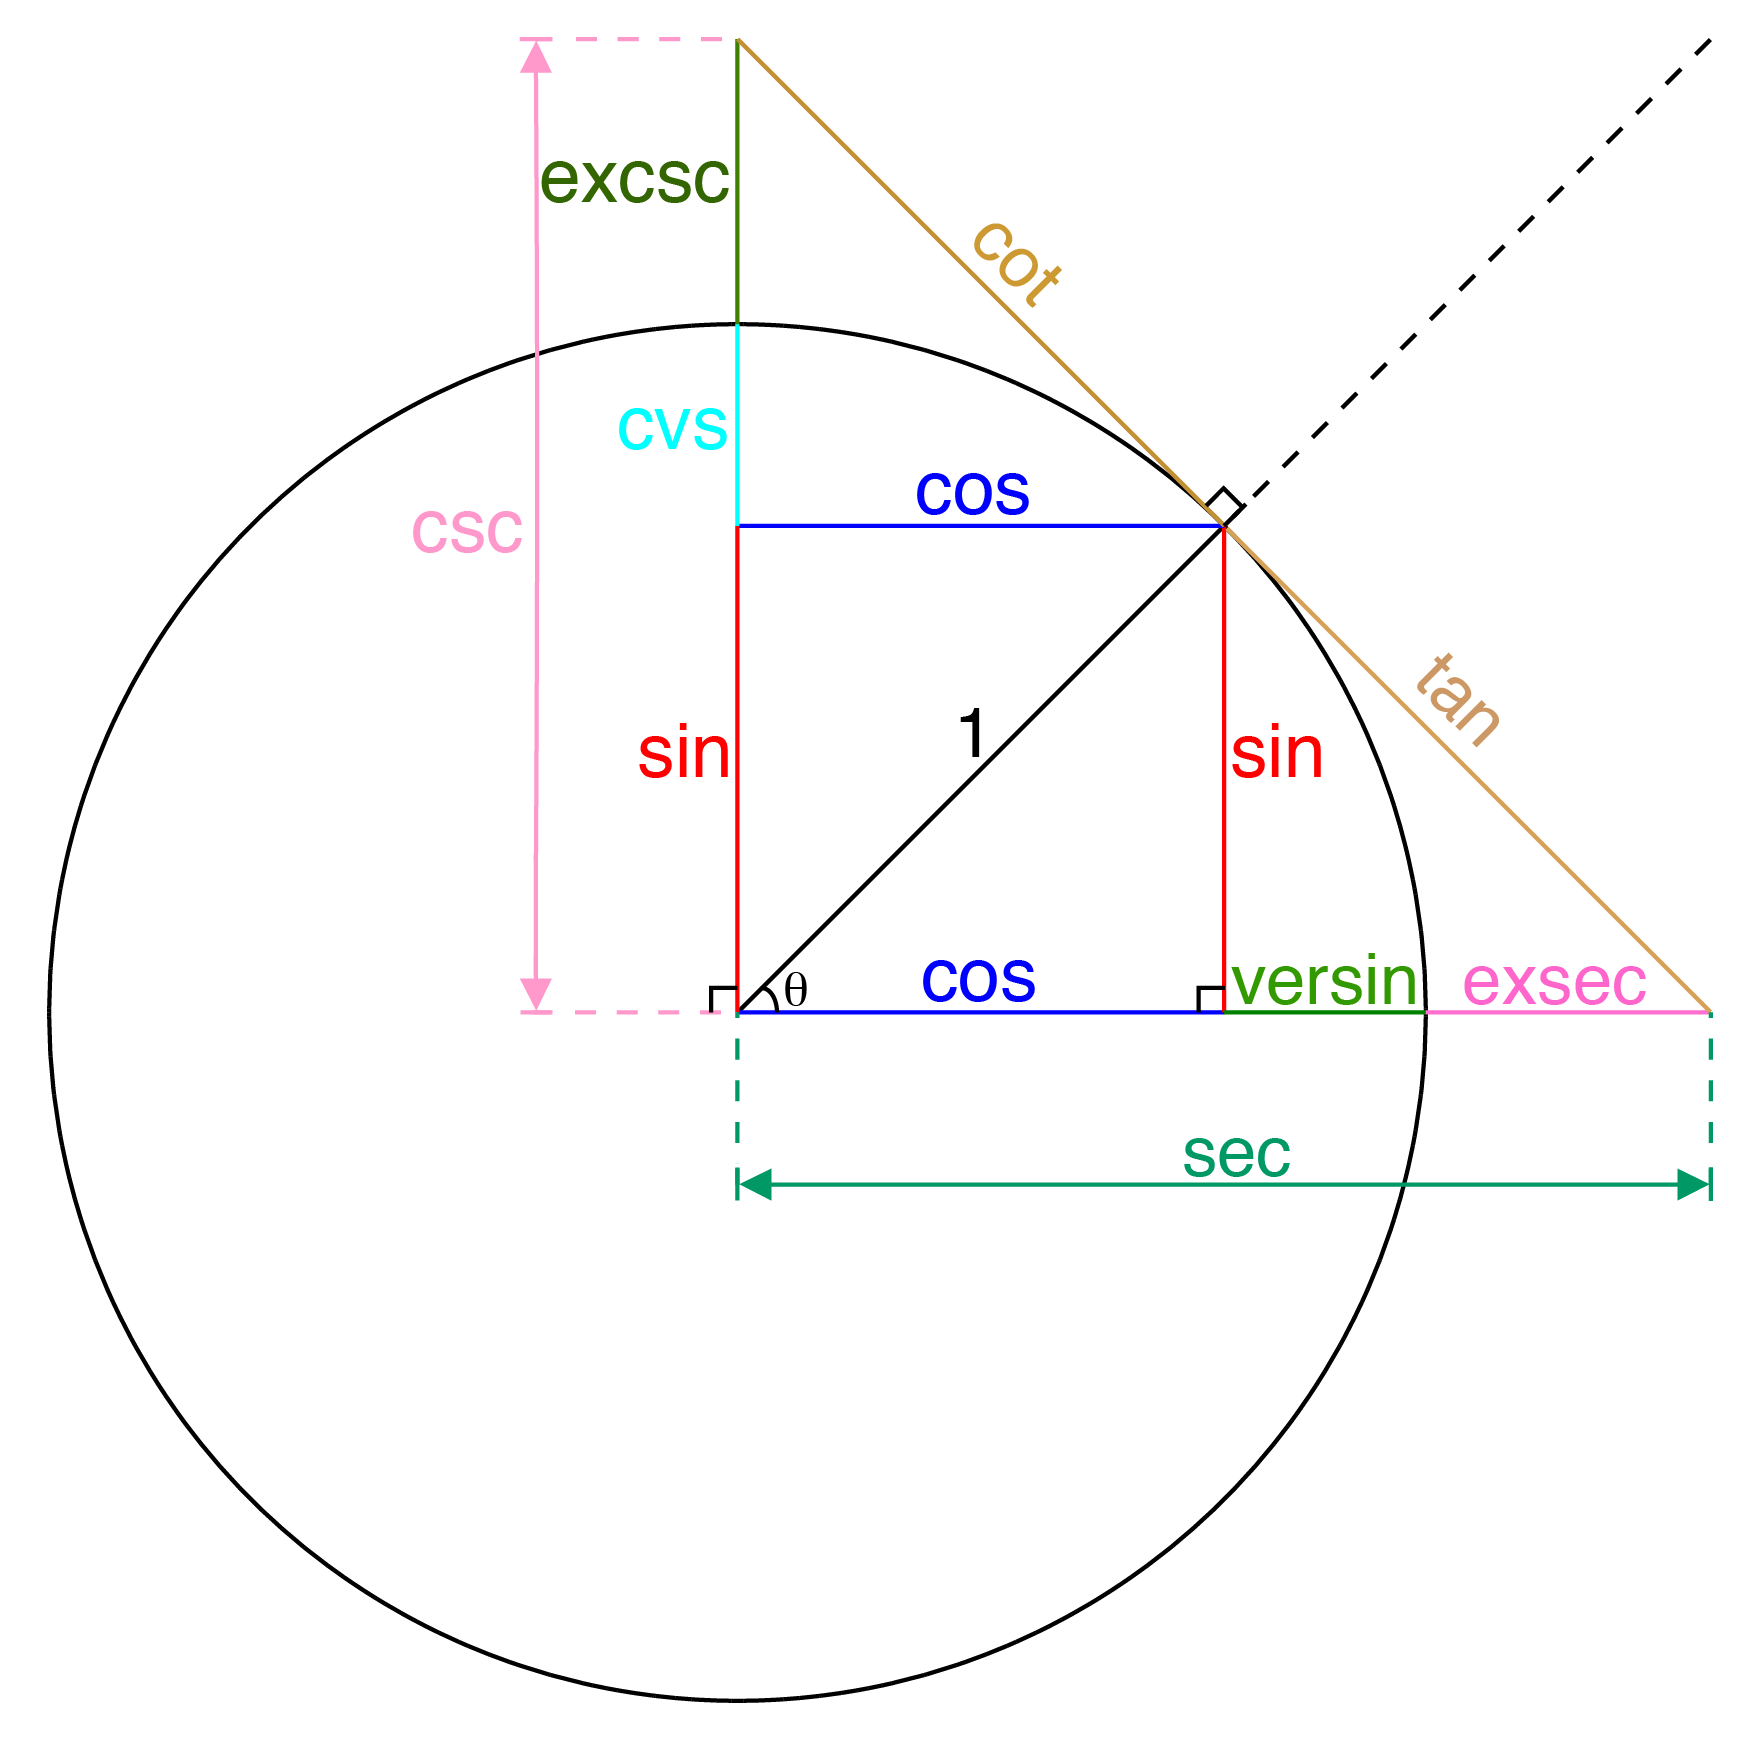
\includegraphics[width=\linewidth]{circle}
	%\captionof{figure}{my caption of the figure}
\end{Figure}
\subsection*{Domain and Range}
\begin{itemize}[leftmargin=0.5em, label={.}]
  \item $\sin: \R \longrightarrow[-1,1]$
  \item $\cos: \R \longrightarrow[-1,1]$
  \item $\tan: \left\{x \in \R \ \middle| \ x \neq \frac{\pi}{2} + k\pi\right\}\longrightarrow\R$
  \item $\cot: \left\{x \in \R \ \middle| \ x \neq k\pi\right\}\longrightarrow\R$
  \item $\csc: \left\{x \in \R \ \middle| \ x \neq k\pi\right\}\longrightarrow \R \setminus \left(-1,1 \right)$
  \item $\sec:\left\{x \in \R \ \middle| \ x \neq \frac{\pi}{2} + k\pi\right\}\longrightarrow \R \setminus \left(-1,1\right)$
  \item $\sin^{-1}: \left[-1,1\right] \longrightarrow \left[-\frac{\pi}{2},\frac{\pi}{2}\right]$
  \item $\cos^{-1}: \left[-1,1\right] \longrightarrow \left[0,\pi\right]$		
  \item $\tan^{-1}: \R \longrightarrow \left[-\frac{\pi}{2},\frac{\pi}{2}\right]$
\end{itemize}

\subsection*{Pythagorean Identities}	
\begin{eqlist}
	\item $\sin^2(x) + \cos^2(x) = 1$
	\item $\tan^2(x) + 1 = \sec^2(x)$
	\item $1 + \cot^2(x) = \csc^2(x)$
\end{eqlist}


\subsection*{Quotient Identities}	
\begin{eqlist}
	\item $\tan(x) = \frac{\sin(x)}{\cos(x)}$
	\item $\cot(x) = \frac{\cos(x)}{\sin(x)}$
        \item $\csc(x) = \frac{1}{\sin(x)}$
        \item $\sec(x) = \frac{1}{\cos(x)}$
\end{eqlist}

\subsection*{Sum Identities}	
\begin{eqlist}
	\item $\sin(x + y) = \sin(x)\cos(y) + \cos(x)\sin(y)$
	\item $\cos(x + y) = \cos(x)\cos(y) - \sin(x)\sin(y)$
	\item $\tan(x + y) = \frac{\tan(x) + \tan(y)}{1-\tan(x)\tan(y)}$
\end{eqlist}

\subsection*{Difference Identities}	
\begin{eqlist}
	\item $\sin(x - y) = \sin(x)\cos(y) - \cos(x)\sin(y)$
	\item $\cos(x - y) = \cos(x)\cos(y) + \sin(x)\sin(y)$
	\item $\tan(x - y) = \frac{\tan(x) - \tan(y)}{1 + \tan(x)\tan(y)}$
\end{eqlist}

\subsection*{Double Angle Identities}	
\begin{eqlist}
	\item $\sin(2x) = 2\sin(x)\cos(x)$
	\item $\cos(2x) = \cos^2(x) - \sin^2(x) $
	\item $\cos(2x) = 2\cos^2(x) - 1$
	\item $\cos(2x) = 1 - 2\sin^2(x)$
	\item $\tan(2x) = \frac{2\tan(x)}{1-\tan^2(x)} $
\end{eqlist}

\subsection*{Co-Function Identities}	
\begin{eqlist}
	\item $\sin\left(\frac{\pi}{2}-x\right) = \cos(x)$
	\item $\cos\left(\frac{\pi}{2}-x\right) = \sin(x)$
	\item $\tan\left(\frac{\pi}{2}-x\right) = \cot(x)$
	\item $\cot\left(\frac{\pi}{2}-x\right) = \tan(x)$
	\item $\csc\left(\frac{\pi}{2}-x\right) = \sec(x)$	
	\item $\sec\left(\frac{\pi}{2}-x\right) = \csc(x)$
\end{eqlist}

\subsection*{Even-Odd Identities}	
\begin{eqlist}
	\item $\sin(-x) = -\sin(x)$
	\item $\cos(-x) = \cos(x)$
	\item $\tan(-x) = -\tan(x)$
	\item $\cot(-x) = -\cot(x)$
	\item $\csc(-x) = -\csc(x)$
	\item $\sec(-x) = \sec(x)$
\end{eqlist}

\subsection*{Half-Angle Identities}	
\begin{eqlist}
	\item $\sin\left(\frac{x}{2}\right) = \pm\sqrt{\frac{1-\cos(x)}{2}}$
	\item $\cos\left(\frac{x}{2}\right) = \pm\sqrt{\frac{1+\cos(x)}{2}}$
	\item $\tan\left(\frac{x}{2}\right) = \pm\sqrt{\frac{1-\cos(x)}{2}}$
	\item $\tan\left(\frac{x}{2}\right) = \frac{1-\cos(x)}{\sin(x)}$
	\item $\tan\left(\frac{x}{2}\right) = \frac{\sin(x)}{1+\cos(x)}$
\end{eqlist}

\subsection*{Sum-to-Product Formulas}
\begin{eqlist}
	\item $\sin(x) + \sin(y) = 2\sin\left(\frac{x+y}{2}\right)\cos\left(\frac{x-y}{2}\right)$
	\item $\sin(x) - \sin(y) = 2\sin\left(\frac{x-y}{2}\right)\cos\left(\frac{x+y}{2}\right)$
	\item $\cos(x) + \cos(y) = 2\cos\left(\frac{x+y}{2}\right)\cos\left(\frac{x-y}{2}\right)$
	\item $\cos(x) - \cos(y) = -2\sin\left(\frac{x+y}{2}\right)\cos\left(\frac{x-y}{2}\right)$
\end{eqlist}

\subsection*{Product-to-Sum Formulas}
\begin{eqlist}
	\item $\sin(x)\sin(y) = \frac{1}{2}\left[\cos(x-y)-\cos(x+y)\right]$
	\item $\cos(x)\cos(y) = \frac{1}{2}\left[\cos(x-y)+\cos(x+y)\right]$
	\item $\sin(x)\cos(y) = \frac{1}{2}\left[\sin(x+y)+\sin(x-y)\right]$
	\item $\cos(x)\sin(y) = \frac{1}{2}\left[\sin(x+y)-\sin(x-y)\right]$
\end{eqlist}


\subsection*{Laws of Sines}
\begin{eqlist}
	\item $\frac{\sin(\alpha)}{a} = \frac{\sin(\beta)}{b} = \frac{\sin(\gamma)}{c}$
\end{eqlist}

\subsection*{Laws of Cosines}
\begin{eqlist}
	\item $a^2 = b^2 + c^2 - 2bc\cos(\alpha)$
	\item $b^2 = a^2 + c^2 - 2ac\cos(\beta)$
	\item $c^2 = a^2 + b^2 - 2ab\cos(\gamma)$
\end{eqlist}

\subsection*{Degrees}
\begin{Figure}
	\centering
	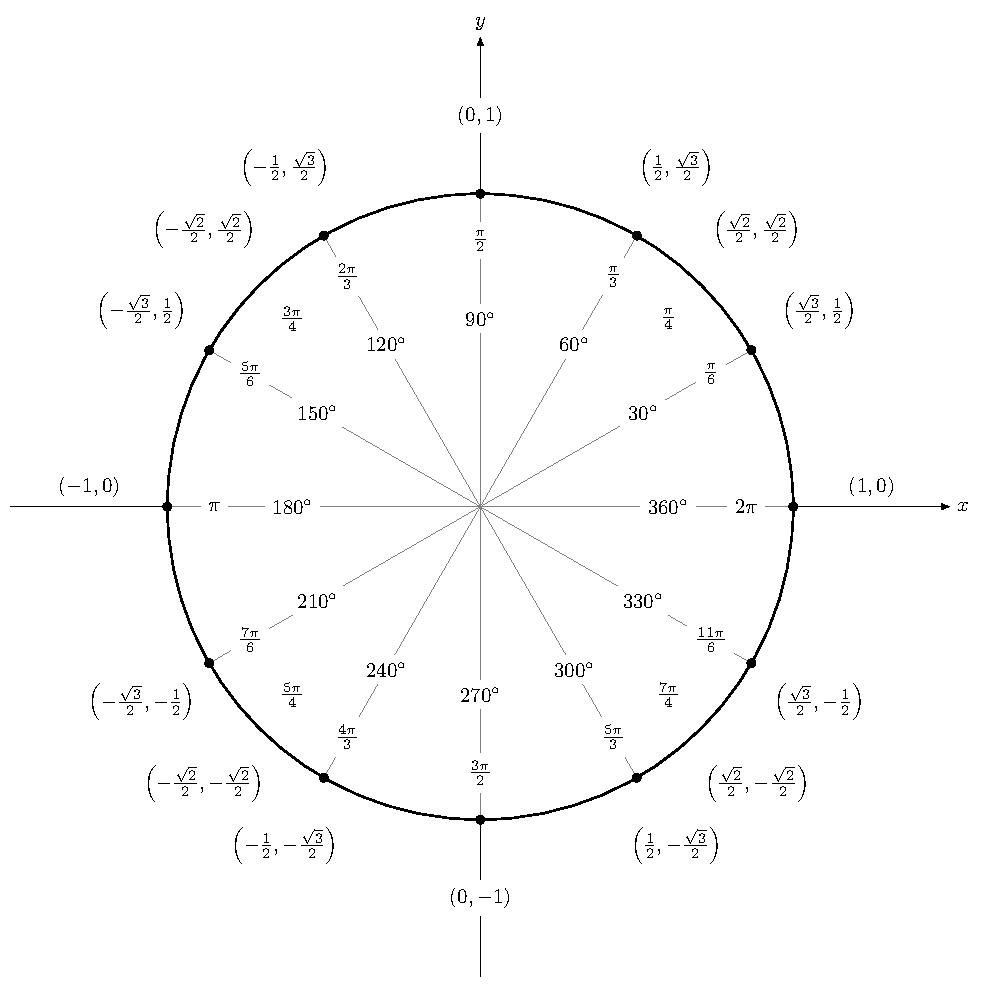
\includegraphics[width=\linewidth]{degrees_circle}
	%\captionof{figure}{my caption of the figure}
\end{Figure}

\begin{Figure}
	\centering
	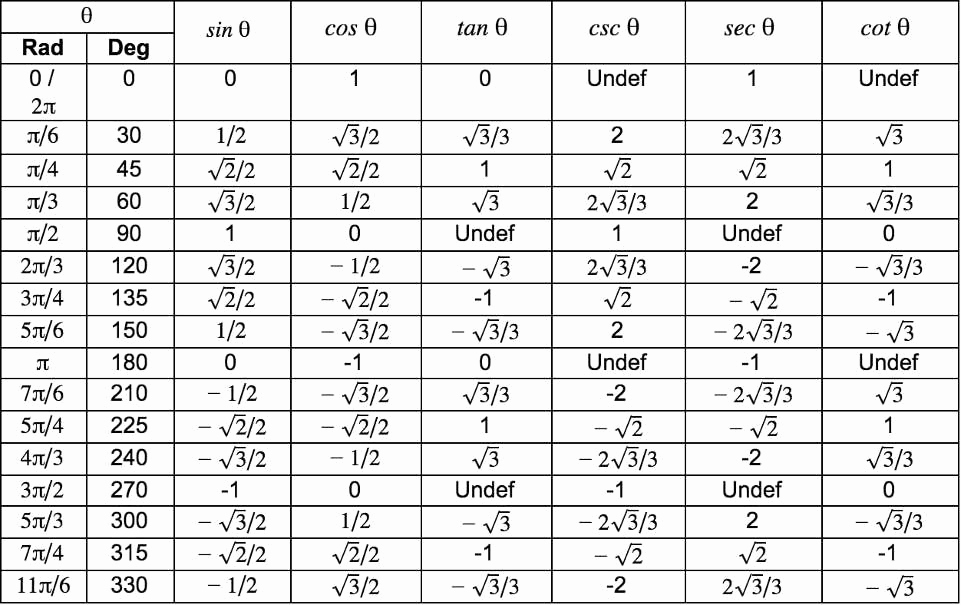
\includegraphics[width=\linewidth]{unit_circle_table}
\end{Figure}


\section*{Unit 1: Limits \& Continuity}
\subsection*{Indeterminate Forms}
Forms of type $\frac{0}{0}$, $\frac{\infty}{\infty}$, $0^\infty$, $\infty^0$, $1^\infty$, $\infty-\infty$ or $0\cdot\left(\pm\infty\right)$


\section*{Unit 2: Differentiation: Fundamental Properties}


\section*{Unit 3: Differentiation: Advanced}


\section*{Unit 4: Contextual Applications of Differentiation}


\section*{Unit 5: Analytical Applications of Differentiation}


\section*{Unit 6: Integration and Accumulation of Change}


\section*{Unit 7: Differential Equations}


\section*{Unit 8: Applications of Integration}


\section*{Unit 9: Parametric Equations, Polar Coordinates, \& Vector-Valued Functions}


\section*{Unit 10: Infinite Sequences \& Series}


\end{multicols}
\end{document}

